\newpage

\subsection{General Purpose Scenarios}\label{ssec:UseCase3-DatasetMGMT}

Unlike the previous use cases, the following two use cases operate on a test graph to demonstrate their purpose. Moreover, they allow to depict an arbitrary amount of information on their cards. 


\subsubsection{Use Case 3: Dataset Management}

This use case is applicable if a user wants to manage the state of existing datasets. The underlying graph is eccenca’s \textit{\tracknshrink{CMEM} Dataset catalog}, which provides a system to manage and govern datasets and resources in eccenca’s \textit{Corporate Memory}.



\vspace*{\baselineskip}

\noindent \textsc{Outline}\\
\noindent In contrast to the previous use cases, these scenarios demand to display arbitrary resources on a card. For example, the \textit{\tracknshrink{CMEM} Dataset catalog} contains two resources which should be depicted on a card, if existing. That is (1) the property \textit{version} that refers to a literal value indicating a dataset’s version number or label, and (2) the property \textit{update frequency}, which refers to a resource indicating a time interval. Ultimately, the scenario’s goal is to visualize datasets and manage their predefined statuses within the \acrshort*{RMB}.  


\vspace*{\baselineskip}

\noindent \textsc{Board Component Resources}\\[-1.5em]

\noindent \hangindent=1.7cm \textit{Cards.}\tabto{1.7cm} Cards represent datasets that are of type dataset. For this example, the card’s class is \url{https://vocab.eccenca.com/dsm/Dataset}.\\[-1.5em]

\noindent \hangindent=1.7cm \textit{Columns.}\tabto{1.7cm} The board’s column property is \url{https://vocab.eccenca.com/dsm/hasStatus} (i.e., the assigned status). The values of this property are representing the columns of the board (e.g., \textit{needs approval}, \textit{published}, etc.).\\[-1.5em]

\noindent \hangindent=1.7cm \textit{Lanes.}\tabto{1.7cm} Datasets are part of a broader domain; for example, a dataset containing personal data may belong to the field of human resources. A property that expresses its affiliation in the context of dataset management is \url{http://www.w3.org/ns/dcat\#theme} from the \textit{Data Catalog Vocabulary} (\tracknshrink{DCAT}) \parencite[]{Erickson2014}, which will be used for this purpose.


\vspace*{\baselineskip}

\noindent \textsc{Card Component Resources}\\
\noindent A card’s title corresponds to a dataset’s \acrshort{rdfs}\texttt{label}. Moreover, as stated above, the cards should depict a list of property-value pairs. In this use case, \textit{version} and \textit{update frequency} are demanded.


\vspace*{\baselineskip}

\noindent \textsc{Mockup}\\
\noindent \autoref{fig:RMB Use Case 3} provides a mockup of the \acrshort*{RMB} with the content requested by the board component and card component resources above. For demonstration purposes, the mockup showcases only three datasets (i.e., \textit{Personal Data}, \textit{Sales Data}, and \textit{\tracknshrink{RND} Spendings} separated by two columns (i.e., the status of the dataset), and two lanes (i.e., the dataset’s domain). In deviation from the previous use cases, the dataset management scenario stresses the application of \textit{additional properties}, which are also depicted on the cards, if they are defined on a resource (i.e., \textit{version} and \textit{update frequency}).

\newpage

\noindent Regarding the goals of this work, this scenario allows to display \acrshort*{RDF} datasets, and to update their status by dragging cards into different columns. For example, a user may intuitively withdraw the dataset \textit{RND Spendings} by dragging the corresponding card from the column \textit{published} to the column \textit{needs approval}, as depicted below.




\begin{figure}[H]
    \libertineLF
    \centering
    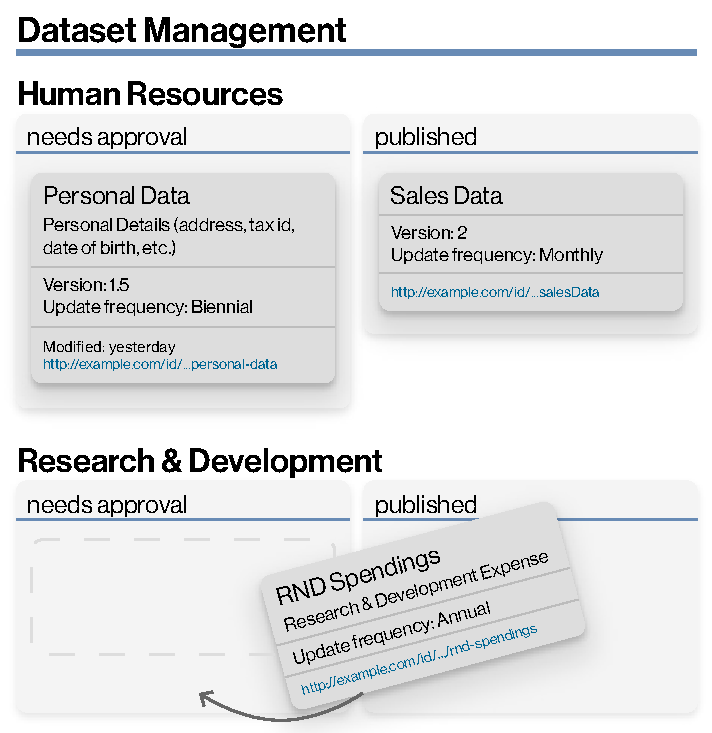
\includegraphics[width=105mm]{img/31-UseCase3.pdf}
	\caption[\tracknshrink{RMB} Mockup of Use Case 3]{\tracknshrink{RMB} Mockup of Use Case 3, including mandatory card elements (i.e., title and resource identifier) and optional elements (i.e., description, additional properties, modified timestamp).}
	\label{fig:RMB Use Case 3}
	\libertineOsF
\end{figure}







